\def\nd{\noindent}
\def\a{\vec{a}}
\def\x{\vec{x}}
\def\y{\vec{y}}
\def\vr{\vec{r}}
\def\n{\vec{n}}
\def\f{\vec{f}}
\def\s{\vec{s}}
\def\p{\partial}
\def\N{\vec{\nabla}}
\def\O{\Omega}
\def\D{ D}
\def\P{ P}

\documentclass[12pt]{article}
\usepackage{hyperref}
\usepackage{amsmath,esint}
%\usepackage{empheq}
\usepackage{amssymb}
%\usepackage{subfigure}
\usepackage{subfig}
\usepackage{graphicx}

\title{ Mesh Generator for Curved Surfaces }

\begin{document}
\maketitle
\tableofcontents
\newpage

%\section*{Nomenclature}
%
%\begin{tabbing}
%XXXXXXXXX \= XXXXXXXXXXXXXXX \kill
%PF \> Propagating Front \\
%\end{tabbing}

\section{Summary}

A mesh generator for creating triangulated representation of curved surface is described. The algorithm takes as an input a set of points on the surface and the corresponding surface-normal vectors and produces the list of surface triangles represented by the triples of node indexes. 

\section{Method}

\subsection{Overview}

Figure~\ref{init_points} shows a typical node distribution provided as an input to the algorithm and Figure~\ref{mesh} shows the meshed surface representation produced by the algorithm.

\begin{figure}
\center
\fbox{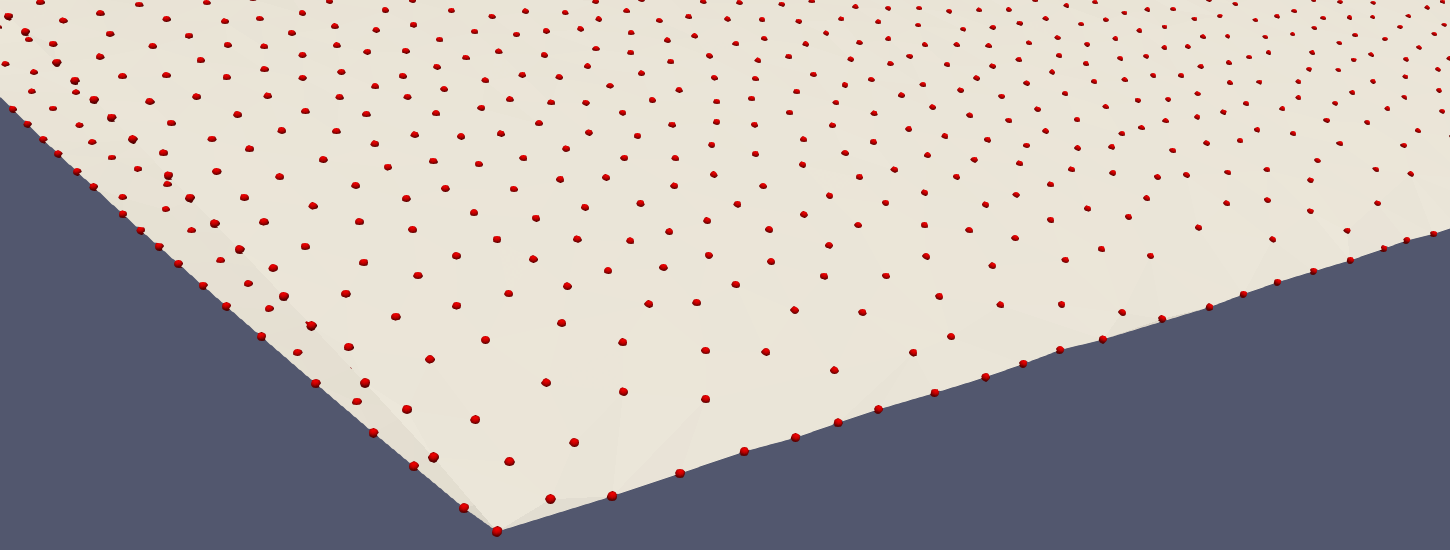
\includegraphics[width=5in]{nodes.png}}
\caption{\label{init_points}Initial points distribution on the surface}
\end{figure}

\begin{figure}
\center
\fbox{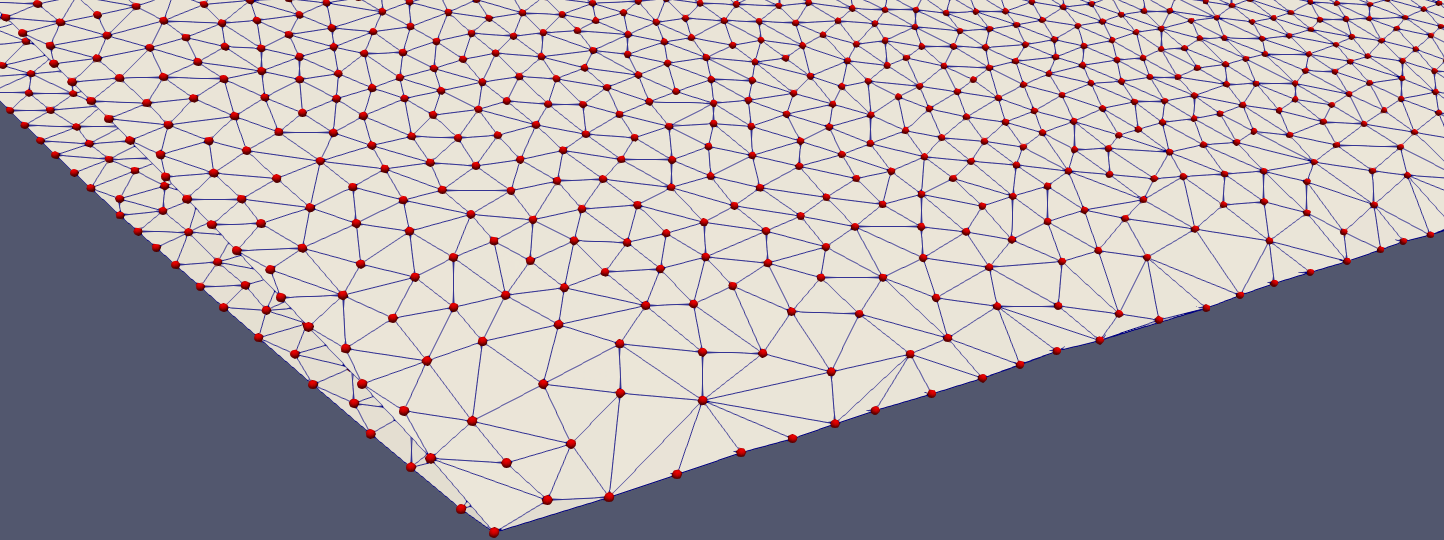
\includegraphics[width=5in]{mesh.png}}
\caption{\label{mesh}Triangulation from the initial set of points}
\end{figure}

The algorithm is based on a propagating-front (PF) method \cite{AkGlCGD2001,OsJCP1988}
with the essential steps shown in Fig.\ref{alg}.

\begin{figure}
\begin{verbatim}
Create the first triangle and assign its edges to PF
WHILE there are still segments in PF DO
| FOR each segment in PF DO
| | Find its closest point
| | IF found THEN
| | | IF the new point belongs to PF THEN
| | | | IF this point is neigboring the current segment THEN
| | | | | IF the point is neibhboring segment on both ends THEN
| | | | | | Add new triangle made of the current segment and 
| | | | | |     its two neighbors
| | | | | | Delete current segment and its neighbors from PF
| | | | | ELSE (point is neighboring on one end only)
| | | | | | Add new mesh triangle at the corner of the segment
| | | | | | Delete current segment and its neighbor from PF
| | | | | | Add one new segment to PF
| | | | ELSE
| | | | | Add new trianle with the segment at its base 
| | | | | Delete current segment from PF
| | | | | Add two side segments to PF
| | | ELSE (the new point does not belong to PF)
| | | | Add new trianle with the segment at its base 
| | | | Delete current segment from PF
| | | | Add two side segments to PF
| | ELSE (point not found)
| | | Assign current segment to the boundary 
| | | Remove current segment from PF
\end{verbatim}
\caption{\label{alg}Propagating Front Algorithm}
\end{figure}

For this algorithm to work on curved surfaces, especially those with sharp
edges, a measure of distance between the points should be modified from the
conventional Euclidean distance to the one appropriate for a curved surface. In
our case we found it convenient to specify a {\em bonding} function between the
points, which represents the strength of connectivity between the points, and
which depends on the positions and surface-normal vectors of the two points. In
particular, the {\em bonding force} between points $A$ and $B$ is calculated
as:

\begin{equation}
\label{bond}
b = \frac{(\vec{N}_A\cdot\vec{N}_B)}{\mid\vec{X}_A-\vec{X}_B\mid}
\end{equation}

\nd
where $\vec{N}$ is the surface normal vector, $\vec{X}$ is the position vector,
$(\cdot)$ is a scalar product between the two vectors and the denominator has the Euclidean
distance between two point positions.  This bonding measure guarantees that
points which can be close together but located on the opposite sides of the
surface will not be considered as being close to each-other.  Thus, a strong
bonding will only be created between the points on the same side of the
surface.  This feature of measuring distance in an expanded space of distances
and surface normals is essential to produces a continuous triangulation on a
highly curved surface.


\subsection{Initializing}

The following data sets are initialized at the beginning of the algorithm:

\begin{enumerate}
\item Points ({\tt points}).
\item Front nodes ({\tt fnodes}).
\item Mesh nodes ({\tt mnodes}).
\item Front segments ({\tt fsegs}).
\item Boundary segments ({\tt bsegs}).
\item Surface mesh triangles ({\tt mesh}).
\end{enumerate}

All the data sets are implemented as doubly linked lists, capable of growing and shrinking as needed. 
The set of points is loaded from the external file, while other data sets are initially empty. 

At the beginning the first triangle is created by selecting a first arbitrary point, finding a second closest point, forming the first segment between the two points, and then picking a third point closest to the middle of the segment.
The three segments forming the first triangle are added to the list of front
segments ({\tt fsegs}) and the three vertices of the triangle are added to the list of front nodes ({\tt fnodes}). After that the triangle is added to the list of mesh triangles ({\tt mesh}).

Then the algorithm starts looping over the list of front segments as long as the list is not empty.

\subsection{Finding Closest Point}

For each segment of the front a middle point of the segment is considered and a
point with the strongest bonding according to (\ref{bond}) is searched
among the lists of free points and among the front nodes. 
To speed up the search only points at locations within a specified
range are considered. That range value can be made dependent on location but
in the current implementation it is constant throughout the domain.

There are two additional constraints applied to candidate points in the bond calculation:

\begin{enumerate}
\item New points should be located ahead of the front.
\item New point should not create intersection with an existing front segment (Fig.\ref{intersect}).
\end{enumerate}

\begin{figure}
\center
\fbox{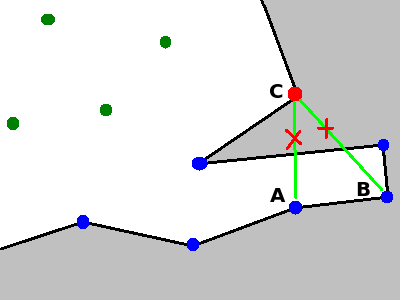
\includegraphics[width=3in]{intersection.png}}
\caption{\label{intersect}New point creates intersection}
\end{figure}

The first constraint is realized by considering only the points which are on
the positive side of the plane formed by the surface normal and the segment
line. The surface normal vectors supplied as input to the algorithm are used
for this purpose.

The second constraint is realized by using standard line intersection algorithm
on a plane adapted for a 3D case by projecting all the points to the plane
perpendicular to the surface normal vector.


After the two searches over two respective lists ({\tt points, bnodes}) are
completed, three possibilities are considered: 
(1) 
there are no candidates for the next mesh node,
(2) 
only one list has a candidate, 
(3) 
both lists have candidates for the next mesh node. 

In the first case the current segment is added to the list of boundary segments
({\tt bsegs}) and is removed from the list of front segments ({\tt fsegs}). In
the second case the only available candidate is considered, and in the last
case the candidate with the strongest bond is considered.

After the candidate point is selected further processing depends on whether
this point is on the front or not.


\subsection{Point is not on the Front}


Fig.\ref{newpoint} shows a typical situation when the point selected for a new triangle does not belong to the current propagating mesh front. In this case two new segments (AC, BC) are created and the current segment (AB) is removed from the front. The resulting triangle ABC is added to the surface mesh.

\begin{figure}
\center
\fbox{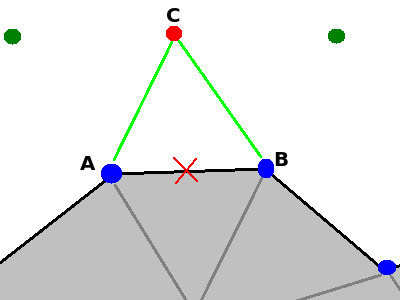
\includegraphics[width=3in]{newpoint.png}}
\caption{\label{newpoint}The closest point (C) is not on the front}
\end{figure}


\subsection{Point is on the Front}

When the selected point is on the front of the mesh, several situations are considered:

\begin{enumerate}

\item {\em The point is not a neighbor of the current front segment} (Fig.\ref{frontfar}).
In this case the new triangle ABC is formed, segment AB is removed from the front, and segments AC and BC are added to the front.

\begin{figure}
\center
\fbox{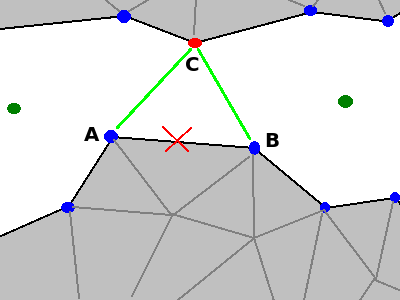
\includegraphics[width=3in]{frontfar.png}}
\caption{\label{frontfar}The closest point (C) on the front is not a neighbor}
\end{figure}

\item {\em The point is a neighbor of the current front segment}
(Fig.\ref{frontneib1}). 
In this case the new triangle ABC is formed, segments AB and BC are removed from the front, and segment AC is added to the front.

\begin{figure}
\center
\fbox{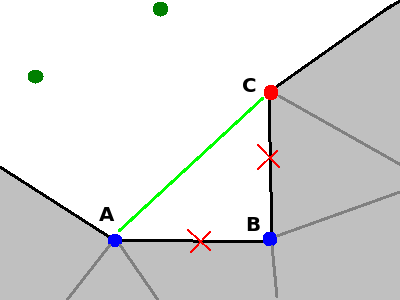
\includegraphics[width=3in]{frontneib1.png}}
\caption{\label{frontneib1}The closest point (C) on the front is also a neighbor}
\end{figure}

\item {\em The point is a neighbor to both vertices of the current segment}
(Fig.\ref{frontneib2}).
This is a case of an isolated triangle. All three segments are removed from the front and the triangle is added to the mesh.


\begin{figure}
\center
\fbox{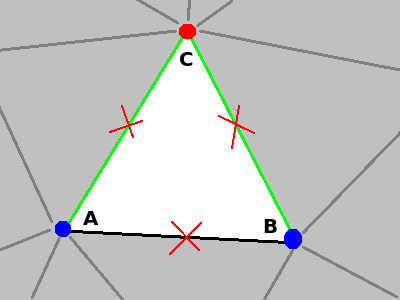
\includegraphics[width=3in]{frontneib2.png}}
\caption{\label{frontneib2}The closest point on the front is a double neighbor}
\end{figure}

\end{enumerate}

\subsection{Closing Gaps}


After the mesh generation is completed, some artificial boundaries can be
produced at sharp edges of the mesh (Fig.\ref{gap}). 
This happens because sharp edges result in boundary segments which can be close
together but don't join since the bonding force between them is too week (i.e.
their surface normals point to the opposite directions). Thus, a separate
routine is needed to mend those holes. This routine loops over all boundary
segments, examines their proximity in Euclidean sense, and joins them if they
are close enough (see Fig.\ref{closegaps}). 

\begin{figure}
\center
\fbox{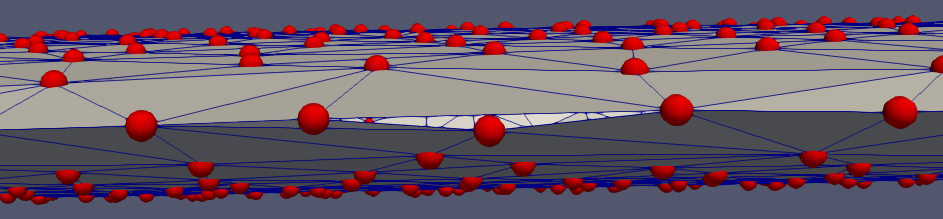
\includegraphics[width=5in]{gap.png}}
\caption{\label{gap}Sharp edges can produce artificial boundaries with gaps}
\end{figure}

\begin{figure}
\center
\fbox{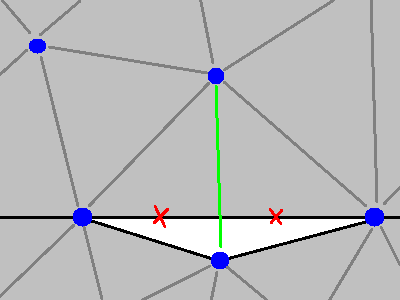
\includegraphics[width=3in]{closegaps.png}}
\caption{\label{closegaps}Closing gaps at the boundaries}
\end{figure}


\section{Source Code}

The source code is written in C++ and is provided in two files: {\tt frontmesh.cc} and {\tt frontmesh.h}.
The former contains implementation of all essential mesh generation functions, while the latter includes description of basic data types such as:
{\tt Vector}, {\tt Point}, {\tt Node}, {\tt Segment}, {\tt Triangle}, and a general {\tt Collection} class to provide link list operations on the basic data types. 
Several global constants defined in {\tt frontmesh.h} file can be used for adjusting the behavior of the algorithm. In particular:

\begin{enumerate}
\item \verb!MIN_ASPECT_RATIO!: the minimum aspec ratio for the triangles.
\item \verb!ZIP_PROXIMITY!: the maximum distance to consider the boundary segments for joining.
\item \verb!RANGE!: the distance beyond which the points are not considered for making a triangle with a current front segment. 
\end{enumerate}

The main routine reads node coordinates and surface normal vectors from text files in Tetgen {\em node} format \cite{TetgenFF} and outputs the resulting node connectivity information in Tetgen {\em face} format.

An additional converter {\tt tetgen2stl} is provided to convert data from Tetgen to STL format.

Detailed information on compiling and running the code is provided in README.md file. Detailed list of data structures is provided in the accompanying code reference manual.



%\hrule
%\newpage
%\bibliographystyle{unsrt}
\bibliographystyle{plain}
\bibliography{surfer}

\end{document}
